\documentclass{article}

\usepackage{graphicx}
\usepackage{tikz}
\usepackage{tikzsymbols}
\usetikzlibrary{calc,patterns,shapes.geometric}
\pagestyle{empty}
\usepackage[margin=0pt]{geometry}
\geometry{papersize={14in,12in}}

\def\centerarc[#1](#2)(#3:#4:#5){\draw[#1] ($(#2)+({#5*cos(#3)},{#5*sin(#3)})$) arc (#3:#4:#5);}

\begin{document}
	\begin{figure}
		\centering
		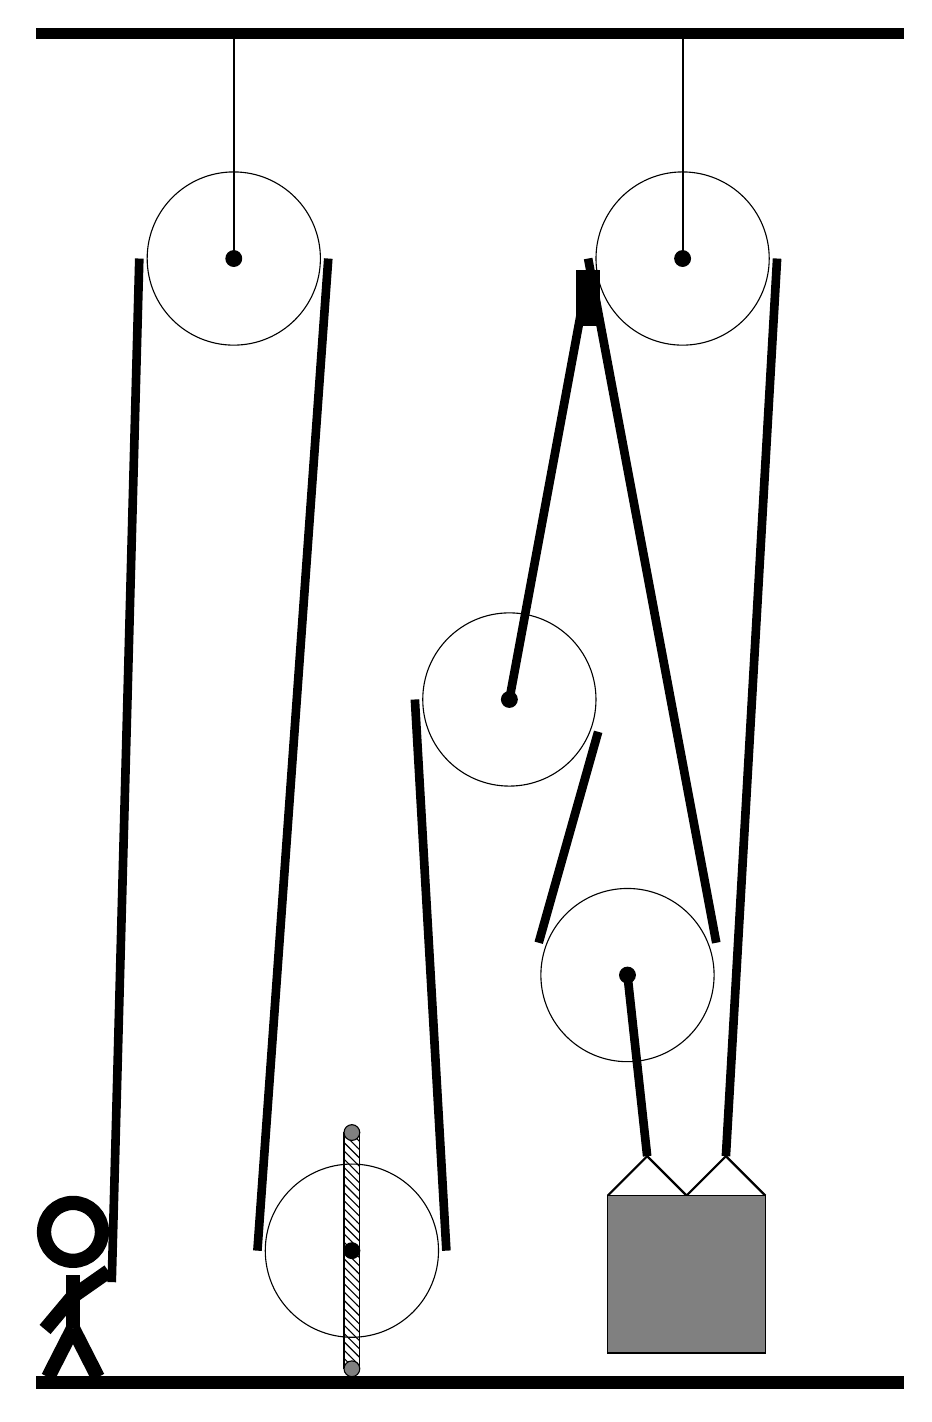
\begin{tikzpicture}
			%%%%% START %%%%%
			\draw[fill=black] (-6, 14) rectangle (5, 14.125);
			
			\draw (0, 5.6) circle (1.1);
			\draw[fill=black] (0, 5.6) circle (0.1);
			
			\draw (1.5, 2.1) circle (1.1);
			\draw[fill=black] (1.5, 2.1) circle (0.1);
			
			\draw (2.2, 11.2) circle (1.1);
			\draw[fill=black] (2.2, 11.2) circle (0.1);
			\draw[thick] (2.2, 11.2) -- (2.2, 14);
			
			\draw (-3.5, 11.2) circle (1.1);
			\draw[fill=black] (-3.5, 11.2) circle (0.1);
			\draw[thick] (-3.5, 11.2) -- (-3.5, 14);
			
			\draw (-2, -1.4) circle (1.1);
			\draw[fill=black] (-2, -1.4) circle (0.1);
			\draw[pattern=north west lines, pattern color=black] (-2.1, 0.1) rectangle (-1.9, -2.9);
			\draw[fill=black!50] (-2, 0.1) circle (0.1);
			\draw[fill=black!50] (-2, -2.9) circle (0.1);
			
			\draw[thick]  (1.25, -0.7) -- (1.75, -0.2) -- (2.25, -0.7) -- (2.75, -0.2) -- (3.25, -0.7);
			\draw[fill=black!50] (1.25, -0.7) rectangle (3.25, -2.7);
			\draw[line width=1.1mm] (-5.05, -1.8) -- (-4.7, 11.2);
			\centerarc[line width=1.1mm](-3.5, 11.2)(0:180:1.2000000000000002);
			\draw[line width=1.1mm] (-2.3, 11.2) -- (-3.2, -1.4);
			\centerarc[line width=1.1mm](-2, -1.4)(180:360:1.2000000000000002);
			\draw[line width=1.1mm] (-0.8, -1.4) -- (-1.2, 5.6);
			\draw[line width=1.1mm] (0, 5.6) -- (1.0, 11.0);
			\draw[line width=1.1mm, fill=black](0.9, 10.4) rectangle (1.1, 11.0);
			\centerarc[line width=1.1mm](0, 5.6)(-20:180:1.2000000000000002);
			\draw[line width=1.1mm] (1.1276, 5.1896) -- (0.3724, 2.5104);
			
			\centerarc[line width=1.1mm](1.5, 2.1)(160:380:1.2000000000000002);
			\draw[line width=1.1mm] (2.6276, 2.5104) -- (1.0, 11.2);
			\draw[line width=1.1mm](1.5, 2.1) -- (1.75, -0.2);
			\centerarc[line width=1.1mm](2.2, 11.2)(0:180:1.2000000000000002);
			\draw[line width=1.1mm] (3.4, 11.2) -- (2.75, -0.2);
			
			\node at (-5.5, -1.9) {\Strichmaxerl[10][50][35]};
			
			\draw[fill=black] (-6, -3) rectangle (5, -3.15);
			%%%%% END %%%%%
		\end{tikzpicture}
	\end{figure}	
\end{document}